\documentclass[openany]{book}
\usepackage{lmodern}
\usepackage{amssymb,amsmath}
\usepackage{ifxetex,ifluatex}
\usepackage{fixltx2e} % provides \textsubscript
\ifnum 0\ifxetex 1\fi\ifluatex 1\fi=0 % if pdftex
  \usepackage[T1]{fontenc}
  \usepackage[utf8]{inputenc}
\else % if luatex or xelatex
  \ifxetex
    \usepackage{mathspec}
  \else
    \usepackage{fontspec}
  \fi
  \defaultfontfeatures{Ligatures=TeX,Scale=MatchLowercase}
\fi
% use upquote if available, for straight quotes in verbatim environments
\IfFileExists{upquote.sty}{\usepackage{upquote}}{}
% use microtype if available
\IfFileExists{microtype.sty}{%
\usepackage{microtype}
\UseMicrotypeSet[protrusion]{basicmath} % disable protrusion for tt fonts
}{}
\usepackage[margin=1in]{geometry}
\usepackage{hyperref}
\hypersetup{unicode=true,
            pdftitle={Finn 6211 - Final Project},
            pdfauthor={mvaugh15@uncc.edu},
            pdfborder={0 0 0},
            breaklinks=true}
\urlstyle{same}  % don't use monospace font for urls
\usepackage{natbib}
\bibliographystyle{apalike}
\usepackage{color}
\usepackage{fancyvrb}
\newcommand{\VerbBar}{|}
\newcommand{\VERB}{\Verb[commandchars=\\\{\}]}
\DefineVerbatimEnvironment{Highlighting}{Verbatim}{commandchars=\\\{\}}
% Add ',fontsize=\small' for more characters per line
\usepackage{framed}
\definecolor{shadecolor}{RGB}{248,248,248}
\newenvironment{Shaded}{\begin{snugshade}}{\end{snugshade}}
\newcommand{\AlertTok}[1]{\textcolor[rgb]{0.94,0.16,0.16}{#1}}
\newcommand{\AnnotationTok}[1]{\textcolor[rgb]{0.56,0.35,0.01}{\textbf{\textit{#1}}}}
\newcommand{\AttributeTok}[1]{\textcolor[rgb]{0.77,0.63,0.00}{#1}}
\newcommand{\BaseNTok}[1]{\textcolor[rgb]{0.00,0.00,0.81}{#1}}
\newcommand{\BuiltInTok}[1]{#1}
\newcommand{\CharTok}[1]{\textcolor[rgb]{0.31,0.60,0.02}{#1}}
\newcommand{\CommentTok}[1]{\textcolor[rgb]{0.56,0.35,0.01}{\textit{#1}}}
\newcommand{\CommentVarTok}[1]{\textcolor[rgb]{0.56,0.35,0.01}{\textbf{\textit{#1}}}}
\newcommand{\ConstantTok}[1]{\textcolor[rgb]{0.00,0.00,0.00}{#1}}
\newcommand{\ControlFlowTok}[1]{\textcolor[rgb]{0.13,0.29,0.53}{\textbf{#1}}}
\newcommand{\DataTypeTok}[1]{\textcolor[rgb]{0.13,0.29,0.53}{#1}}
\newcommand{\DecValTok}[1]{\textcolor[rgb]{0.00,0.00,0.81}{#1}}
\newcommand{\DocumentationTok}[1]{\textcolor[rgb]{0.56,0.35,0.01}{\textbf{\textit{#1}}}}
\newcommand{\ErrorTok}[1]{\textcolor[rgb]{0.64,0.00,0.00}{\textbf{#1}}}
\newcommand{\ExtensionTok}[1]{#1}
\newcommand{\FloatTok}[1]{\textcolor[rgb]{0.00,0.00,0.81}{#1}}
\newcommand{\FunctionTok}[1]{\textcolor[rgb]{0.00,0.00,0.00}{#1}}
\newcommand{\ImportTok}[1]{#1}
\newcommand{\InformationTok}[1]{\textcolor[rgb]{0.56,0.35,0.01}{\textbf{\textit{#1}}}}
\newcommand{\KeywordTok}[1]{\textcolor[rgb]{0.13,0.29,0.53}{\textbf{#1}}}
\newcommand{\NormalTok}[1]{#1}
\newcommand{\OperatorTok}[1]{\textcolor[rgb]{0.81,0.36,0.00}{\textbf{#1}}}
\newcommand{\OtherTok}[1]{\textcolor[rgb]{0.56,0.35,0.01}{#1}}
\newcommand{\PreprocessorTok}[1]{\textcolor[rgb]{0.56,0.35,0.01}{\textit{#1}}}
\newcommand{\RegionMarkerTok}[1]{#1}
\newcommand{\SpecialCharTok}[1]{\textcolor[rgb]{0.00,0.00,0.00}{#1}}
\newcommand{\SpecialStringTok}[1]{\textcolor[rgb]{0.31,0.60,0.02}{#1}}
\newcommand{\StringTok}[1]{\textcolor[rgb]{0.31,0.60,0.02}{#1}}
\newcommand{\VariableTok}[1]{\textcolor[rgb]{0.00,0.00,0.00}{#1}}
\newcommand{\VerbatimStringTok}[1]{\textcolor[rgb]{0.31,0.60,0.02}{#1}}
\newcommand{\WarningTok}[1]{\textcolor[rgb]{0.56,0.35,0.01}{\textbf{\textit{#1}}}}
\usepackage{longtable,booktabs}
\usepackage{graphicx,grffile}
\makeatletter
\def\maxwidth{\ifdim\Gin@nat@width>\linewidth\linewidth\else\Gin@nat@width\fi}
\def\maxheight{\ifdim\Gin@nat@height>\textheight\textheight\else\Gin@nat@height\fi}
\makeatother
% Scale images if necessary, so that they will not overflow the page
% margins by default, and it is still possible to overwrite the defaults
% using explicit options in \includegraphics[width, height, ...]{}
\setkeys{Gin}{width=\maxwidth,height=\maxheight,keepaspectratio}
\IfFileExists{parskip.sty}{%
\usepackage{parskip}
}{% else
\setlength{\parindent}{0pt}
\setlength{\parskip}{6pt plus 2pt minus 1pt}
}
\setlength{\emergencystretch}{3em}  % prevent overfull lines
\providecommand{\tightlist}{%
  \setlength{\itemsep}{0pt}\setlength{\parskip}{0pt}}
\setcounter{secnumdepth}{5}
% Redefines (sub)paragraphs to behave more like sections
\ifx\paragraph\undefined\else
\let\oldparagraph\paragraph
\renewcommand{\paragraph}[1]{\oldparagraph{#1}\mbox{}}
\fi
\ifx\subparagraph\undefined\else
\let\oldsubparagraph\subparagraph
\renewcommand{\subparagraph}[1]{\oldsubparagraph{#1}\mbox{}}
\fi

%%% Use protect on footnotes to avoid problems with footnotes in titles
\let\rmarkdownfootnote\footnote%
\def\footnote{\protect\rmarkdownfootnote}

%%% Change title format to be more compact
\usepackage{titling}

% Create subtitle command for use in maketitle
\newcommand{\subtitle}[1]{
  \posttitle{
    \begin{center}\large#1\end{center}
    }
}

\setlength{\droptitle}{-2em}

  \title{Finn 6211 - Final Project}
    \pretitle{\vspace{\droptitle}\centering\huge}
  \posttitle{\par}
  \subtitle{Davis Vaughan}
  \author{\href{mailto:mvaugh15@uncc.edu}{\nolinkurl{mvaugh15@uncc.edu}}}
    \preauthor{\centering\large\emph}
  \postauthor{\par}
      \predate{\centering\large\emph}
  \postdate{\par}
    \date{2018-05-03}

\usepackage{booktabs}
\usepackage{float}

\usepackage{amsthm}
\newtheorem{theorem}{Theorem}[chapter]
\newtheorem{lemma}{Lemma}[chapter]
\newtheorem{corollary}{Corollary}[chapter]
\newtheorem{proposition}{Proposition}[chapter]
\newtheorem{conjecture}{Conjecture}[chapter]
\theoremstyle{definition}
\newtheorem{definition}{Definition}[chapter]
\theoremstyle{definition}
\newtheorem{example}{Example}[chapter]
\theoremstyle{definition}
\newtheorem{exercise}{Exercise}[chapter]
\theoremstyle{remark}
\newtheorem*{remark}{Remark}
\newtheorem*{solution}{Solution}
\begin{document}
\maketitle

{
\setcounter{tocdepth}{1}
\tableofcontents
}
\hypertarget{titlepage}{%
\chapter{Introduction}\label{titlepage}}

This is the final project of Finn 6211, with the intention of getting
comfortable with spot rate data, their relation to yield curve factors,
and various hedging strategies.

The entire analysis, including the code and the report, can be found at
\url{https://github.com/DavisVaughan/final-project-book}. An HTML
version of the report is hosted at
\url{http://final-project-finn-6211.davisvaughan.com/}, and may be
preferable to the PDF version, which can be found at
\url{http://final-project-finn-6211.davisvaughan.com/final-project-book.pdf}.

An R package has been created to accompany the report. It contains a
number of helper functions for cleaning data, manipulating the time
series, and creating the hedging strategies. The package is named
\texttt{ratekit} and can be found on GitHub at
\url{https://github.com/DavisVaughan/ratekit}.

The structure of the report is as follows. Chapter 2 is dedicated to
retrieving and cleaning the data. Chapter 3 is focused on the
calculation of features used in the questions. Chapters 4, 5, and 6
answer the three questions required in the report.

The code used to create the analysis is split into two places. In the
\texttt{R/} folder of the attached zip file are the files used for
downloading the data, cleaning it, and creating the fixed income
features. The actual analysis and answering of the questions is done
inside the \texttt{.Rmd} files found in the top level of the zip file.

This report was written with
\href{https://bookdown.org/yihui/bookdown/}{bookdown}, a book authoring
package for R.

\small

\normalsize

\hypertarget{data}{%
\chapter{Data}\label{data}}

\hypertarget{retrieve}{%
\section{Data Retrieval}\label{retrieve}}

The data is retrieved from the Federal Reserve website, under the
discussion series: \emph{The U.S. Treasury Yield Curve: 1961 to the
Present}. The link for that site is:
\url{https://www.federalreserve.gov/pubs/feds/2006/200628/200628abs.html}.
The specific data set downloaded was the XLS file included on the site.
\texttt{ratekit} provides the \texttt{download\_rates\_xls()} helper
function for this.

The data was immediately opened in Excel, and resaved as an
\texttt{xlsx} file. The format of the raw data is not a true
\texttt{xls} file, rather, it is some flavor of an \texttt{xml} file.
This does not play nicely with R's packages for importing Excel data, so
a resave was necessary and is done manually.

\hypertarget{cleaning}{%
\section{Cleaning}\label{cleaning}}

Data is brought into R using the \texttt{readxl} package and the
\texttt{ratekit} helper, \texttt{read\_rates()}. This function sets any
\texttt{-999.99} values to \texttt{NA}. These are often found through
the dataset, especially in the parameters columns, and it is assumed
that they represent missing values.

\small

\normalsize

The column names in the data correspond to different types and lengths
of rates used in the paper, along with the names of the parameters in
the model. The key for understanding the column names is shown in Table
\ref{tab:meta}.

\small

\begin{table}[H]

\caption{\label{tab:meta}Rates data: Column key}
\centering
\begin{tabular}[t]{lll}
\toprule
Series & Compounding Convention & Key\\
\midrule
Zero-coupon yield & Continuously Compounded & SVENYXX\\
Par yield & Coupon-Equivalent & SVENPYXX\\
Instantaneous forward rate & Continuously Compounded & SVENFXX\\
One-year forward rate & Coupon-Equivalent & SVEN1FXX\\
Parameters & NA & BETA0 to TAU2\\
\bottomrule
\end{tabular}
\end{table}

\normalsize

Most of these columns are not important for this analysis. Only the
parameter columns and the date column are kept. To further examine the
missing values, the \texttt{skimr} package was used, producing the
report shown below. The \texttt{TAU2} column has a number of missing
values (resulting from either being missing or from being
\texttt{-999.99} values assumed to be missing). All of them occur before
1980, and were removed from the data set. After that removal, no missing
values remain, and the values for the other parameters seemed to
stabilize as well.

\small

Skim summary statistics\\
n obs: 14163\\
n variables: 7

Variable type: Date

\begin{tabular}{llllllll}
\toprule
variable & missing & complete & n & min & max & median & n\_unique\\
\midrule
date & 0 & 14163 & 14163 & 1961-06-14 & 2018-03-29 & 1989-11-10 & 14163\\
\bottomrule
\end{tabular}

Variable type: numeric

\begin{tabular}{lllllllllll}
\toprule
variable & missing & complete & n & mean & sd & p0 & p25 & p50 & p75 & p100\\
\midrule
BETA0 & 0 & 14163 & 14163 & 5.88 & 4.63 & 0 & 3.03 & 5.01 & 7.92 & 25\\
BETA1 & 0 & 14163 & 14163 & -0.82 & 5.05 & -39.73 & -3.07 & -1.02 & 1.41 & 97.18\\
BETA2 & 0 & 14163 & 14163 & -341.06 & 5684.56 & -340683.77 & -9.02 & -0.99 & 1.93 & 94.87\\
BETA3 & 0 & 14163 & 14163 & 343.72 & 5684.31 & -104.03 & 0 & 3.72 & 18.81 & 340681.5\\
TAU1 & 0 & 14163 & 14163 & 2.39 & 3.37 & 0.1 & 0.63 & 1.47 & 2.65 & 30\\
TAU2 & 4620 & 9543 & 14163 & 8.97 & 7.64 & 0.1 & 3.52 & 8.94 & 13.06 & 180.86\\
\bottomrule
\end{tabular}

\normalsize

\hypertarget{monthly}{%
\section{Monthly and Ascending}\label{monthly}}

\small

\normalsize

Monthly data is required for the report, but daily data is provided from
the Federal Reserve data set. The data is converted to monthly
(end-of-month) using the \texttt{tibbletime} package. This leaves 459
rows of data for the project, spanning 1980-01-31 to 2018-03-29.

\small

\normalsize

\hypertarget{rates}{%
\chapter{Fixed Income Features Calculations}\label{rates}}

In this chapter, the construction of spot rates, zero coupon bond
prices, excess returns, and yield factors are discussed. These features
are used in hedging strategies and for general exploration of the data
in Chapters 4-5, so only the implementation is discussed here.

\small

\normalsize

\hypertarget{spot-rates}{%
\section{Spot Rates}\label{spot-rates}}

Spot rates series can be constructed from the 6 parameters in the
cleaned Federal Reserve data set. The following formula is used to
construct the spot rates. It is integrated form of the Svensson
extension of the Nelson and Siegal approach to calculating instantaneous
forward rates. Svensson added a second hump term to the model that
Nelson and Siegal created. Integrating the instantaneous forward rates
gives us the spot rates.

\[
\begin{aligned}
  y_t(n) &= \beta_{0,t} \\
   &+ \beta_{1,t} \frac{1 - \exp(- \frac{n}{\tau_{1,t}})}{\frac{n}{\tau_{1,t}}} \\
   &+ \beta_{2,t} [\frac{1 - \exp(- \frac{n}{\tau_{1,t}})}{\frac{n}{\tau_{1,t}}} - \exp(-\frac{n}{\tau_{1,t}})] \\
   &+ \beta_{3,t} [\frac{1 - \exp(- \frac{n}{\tau_{2,t}})}{\frac{n}{\tau_{2,t}}} - \exp(-\frac{n}{\tau_{2,t}})]
\end{aligned}
\]

Spot rates are examined in detail in Chapter \ref{q1}, but Figure
\ref{fig:spot-rate-time-series} provides a quick look at the major ones.
As expected, longer maturity spot rates are consistently higher than
short term spot rates. The 1980's were a time of incredibly high
interest rates, and in recent years rates have been incredibly low.

\small

\begin{figure}[H]

{\centering 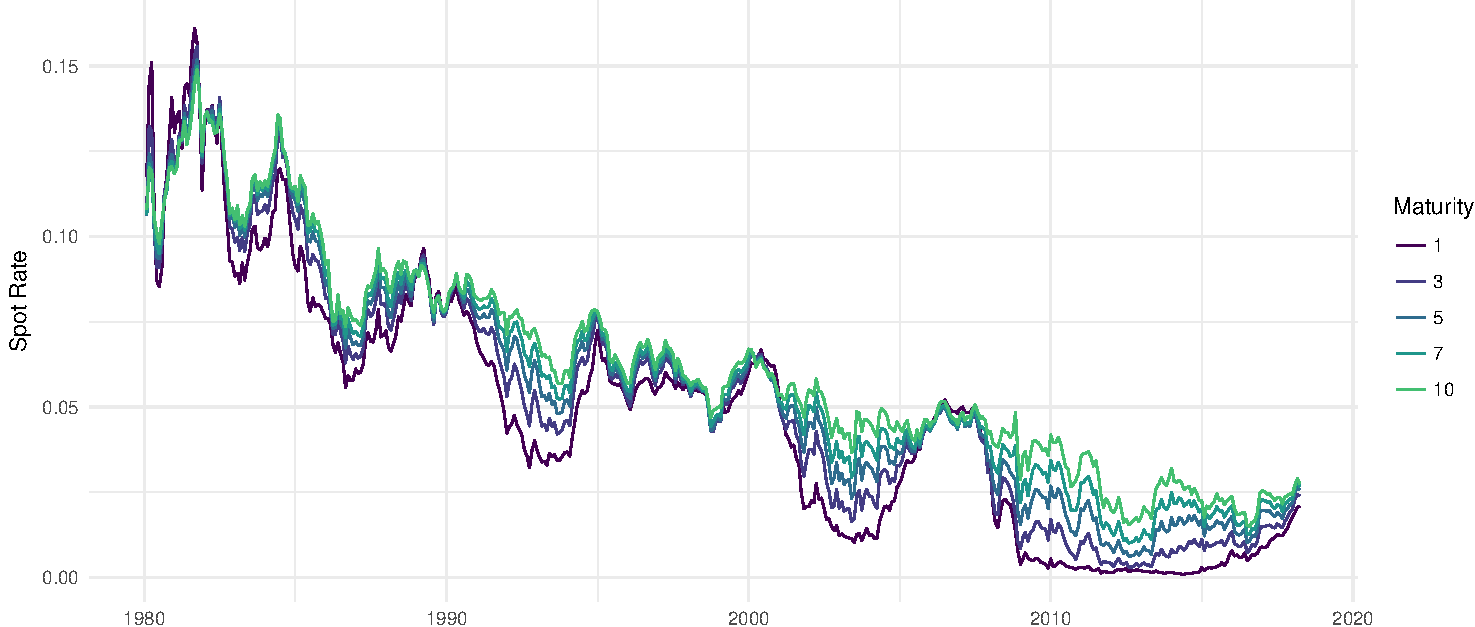
\includegraphics{final-project-book_files/figure-latex/spot-rate-time-series-1} 

}

\caption{Spot rates at various maturities from 1980 onward.}\label{fig:spot-rate-time-series}
\end{figure}

\normalsize

\hypertarget{zero-prices}{%
\section{Zero Coupon Bond Prices}\label{zero-prices}}

N-year zero coupon bond prices can be calculated easily from their
corresponding spot rates. The following formula is used to represent the
relationship between the two series.

\[ P_t(n) = \exp(-y_t(n) \times n) \]

Zero prices, by design, exhibit an inverse relationship to spot rates.
The impact of the high interest rates in the 1980's can be seen clearly
in Figure \ref{fig:zero-prices-time-series}, with a large price spread
between the short and long term maturity zeroes.

\small

\begin{figure}[H]

{\centering 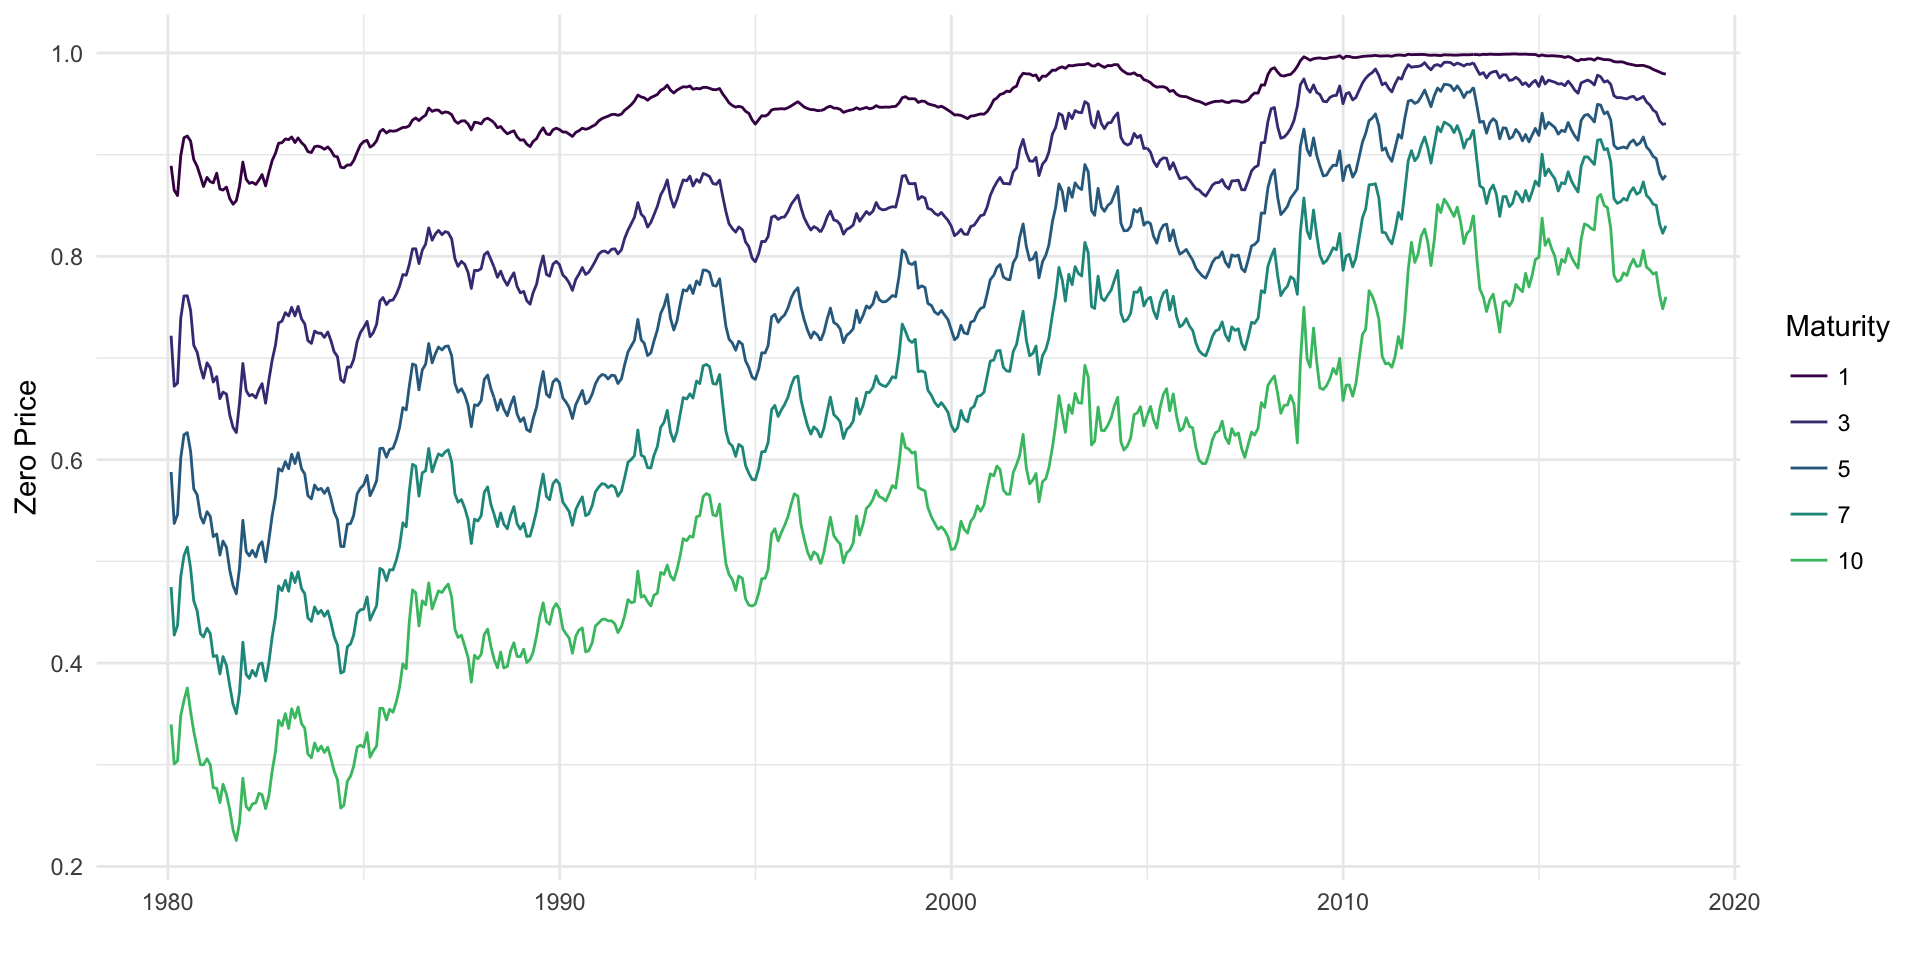
\includegraphics{final-project-book_files/figure-latex/zero-prices-time-series-1} 

}

\caption{Zero prices at various maturities from 1980 onward.}\label{fig:zero-prices-time-series}
\end{figure}

\normalsize

\hypertarget{one-month-returns}{%
\section{One Month Returns}\label{one-month-returns}}

The time \(t+\Delta\) return on an n-year bond is defined as:

\[ RET_{t+\Delta}(n) = \frac{P_{t+\Delta}(n - \Delta)}{P_t(n)} - 1 \]

Using the zero coupon bond prices from Section \ref{zero-prices}, it is
straightforward to calculate returns. Care must be taken to align the
price from next month's \(n-\Delta\) maturity bond with today's \(n\)
maturity bond, but otherwise the procedure is simple.

The distribution of 1-month (\(\Delta = 1/12\)) returns is shown in
Figure \ref{fig:returns-dist}. As seen in both the figure and Table
\ref{tab:returns-summary}, higher maturity zeros have both larger
average returns and more variance. In general, this is unsurprising, and
the drop in standard deviation is roughly linear as the maturity
decreases.

\small

\begin{figure}[H]

{\centering 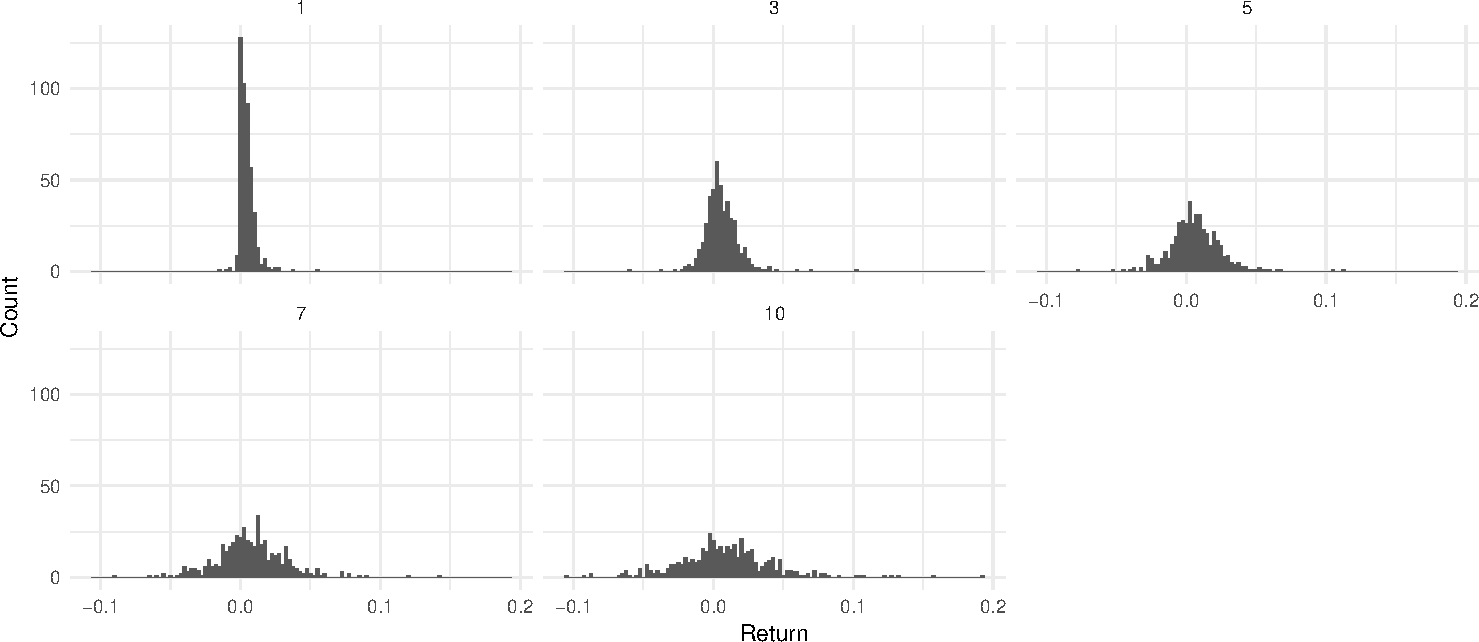
\includegraphics{final-project-book_files/figure-latex/returns-dist-1} 

}

\caption{Return distributions for various maturities.}\label{fig:returns-dist}
\end{figure}

\normalsize

\small

\begin{table}[H]

\caption{\label{tab:returns-summary}Summary statistics of zero coupon bond returns since the 1980's.}
\centering
\begin{tabular}[t]{lrr}
\toprule
Maturity & Average Return & Standard Deviation\\
\midrule
1 & 0.0044510 & 0.0056046\\
3 & 0.0055643 & 0.0125839\\
5 & 0.0064662 & 0.0188464\\
7 & 0.0072532 & 0.0250410\\
10 & 0.0083056 & 0.0343082\\
\bottomrule
\end{tabular}
\end{table}

\normalsize

\hypertarget{excess-returns}{%
\section{Excess Returns}\label{excess-returns}}

Excess returns are calculated over the 1 month treasury, specifically:

\[ ER_{t+\Delta}(n) = RET_{t+\Delta}(n) - RET_{t+\Delta}(\Delta) \]

with \(\Delta = 1 / 12\). Excess returns are only calculated for
\(n = 1, 3, 5, 7, \text{and } 10\) year zeros.

The implementation of this is straightforward since returns for all
maturities have already been calculated. Excess returns show a similar
distribution as returns, just shifted downwards by the 1-month treasury
return.

\hypertarget{yield-curve-factors}{%
\section{Yield Curve Factors}\label{yield-curve-factors}}

Finally, the yield curve factors, level, slope, and curvature are
calculated as:

\[
\begin{aligned}
  \text{Level} &= y_t(1/4) \\
   \text{Slope} &= y_t(8) - y_t(1/4) \\
   \text{Curvature} &= [ y_t(8) - y_t(2) ]  - [ y_t(2) - y_t(1/4) ]
\end{aligned}
\] As seen in Figure \ref{fig:yield-factors}, the raw values of the
yield curve factors do not offer much insight on their own, but they
will be useful later in decomposing the spot rate and in multiplicative
regression hedging.

\small

\begin{figure}[H]

{\centering 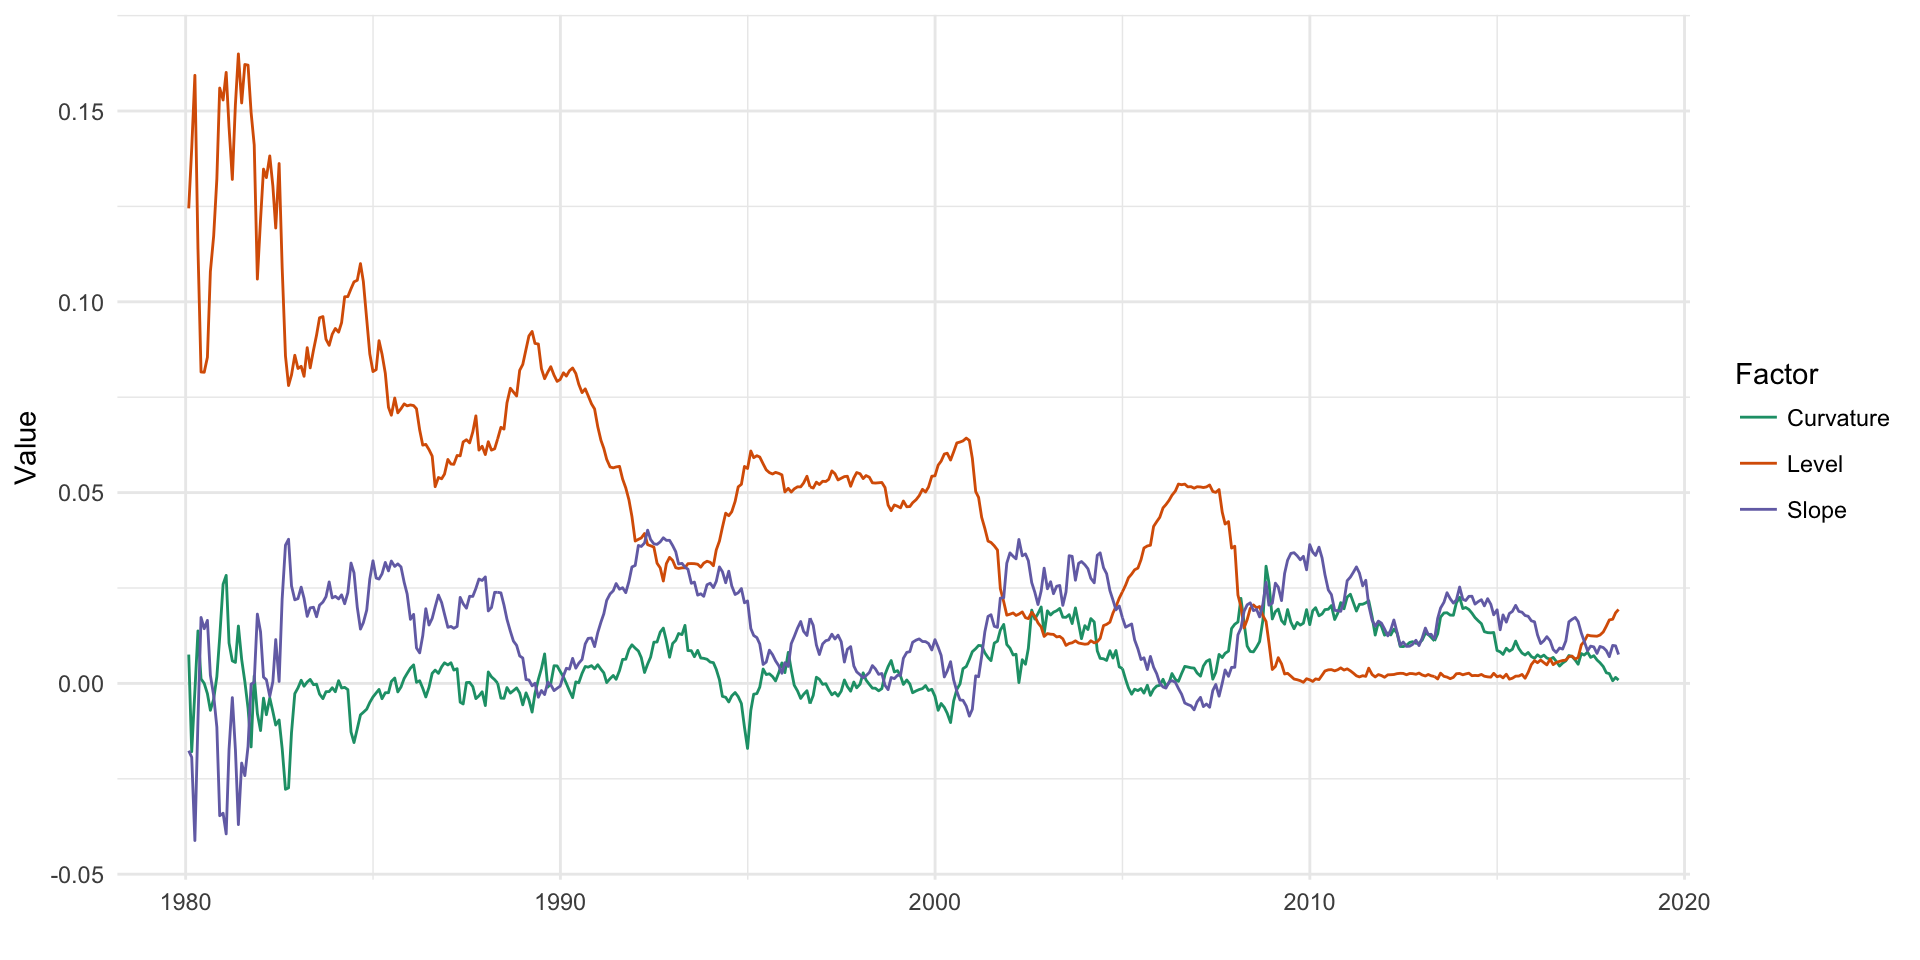
\includegraphics{final-project-book_files/figure-latex/yield-factors-1} 

}

\caption{Yield curve factors over time.}\label{fig:yield-factors}
\end{figure}

\normalsize

\small

\normalsize

\hypertarget{q1}{%
\chapter{Question 1}\label{q1}}

\textbf{Question:}

\emph{What are the time-series properties of the spot rates \(y_t(1)\),
\(y_t(5)\), and \(y_t(10)\)? Report their summary statistics, including
mean, standard deviation, skewness, kurtosis, and the first four
autocorrelation coefficients, and the correlation matrix of the spot
rates. Comment on your results. Also plot them and comment on the time
series patterns.}

\small

\normalsize

In this question, data for the \(y_t(1)\), \(y_t(5)\), and \(y_t(10)\)
spot rates is required. This has been calculated in Section
\ref{spot-rates}, and the results from there are used here.

\small

\normalsize

\hypertarget{summary-statistics}{%
\section{Summary Statistics}\label{summary-statistics}}

Reported in Table \ref{tab:spot-rate-summary} are summary statistics on
the three spot rate series. Unsurprisingly, the average spot rate
increases with the maturity, but interestingly, the shorter maturity
spot rates have higher volatility. The kurtosis of all three are less
than that of a normal distribution, but the 1-year maturity is very
close. All three are right-skewed, with longer right tails, which makes
sense considering extremely high interest rate periods do happen, but
are rare. The histograms in Figure \ref{fig:spot-rate-hist} are a nice
visual confirmation of the results in the table. The skewness is clear,
and the higher standard deviation for lower maturities might be
attributed to the higher density at the extreme tails.

\small

\begin{table}[H]

\caption{\label{tab:spot-rate-summary}Summary statistics for 1, 5, and 10 year spot rates.}
\centering
\begin{tabular}[t]{rrrrr}
\toprule
Maturity & Mean & Standard Deviation & Kurtosis & Skewness\\
\midrule
1 & 0.0480538 & 0.0375029 & 2.913858 & 0.6505396\\
5 & 0.0566592 & 0.0345430 & 2.567191 & 0.5659543\\
10 & 0.0627654 & 0.0314939 & 2.586681 & 0.5793584\\
\bottomrule
\end{tabular}
\end{table}

\normalsize

\small

\begin{figure}[H]

{\centering 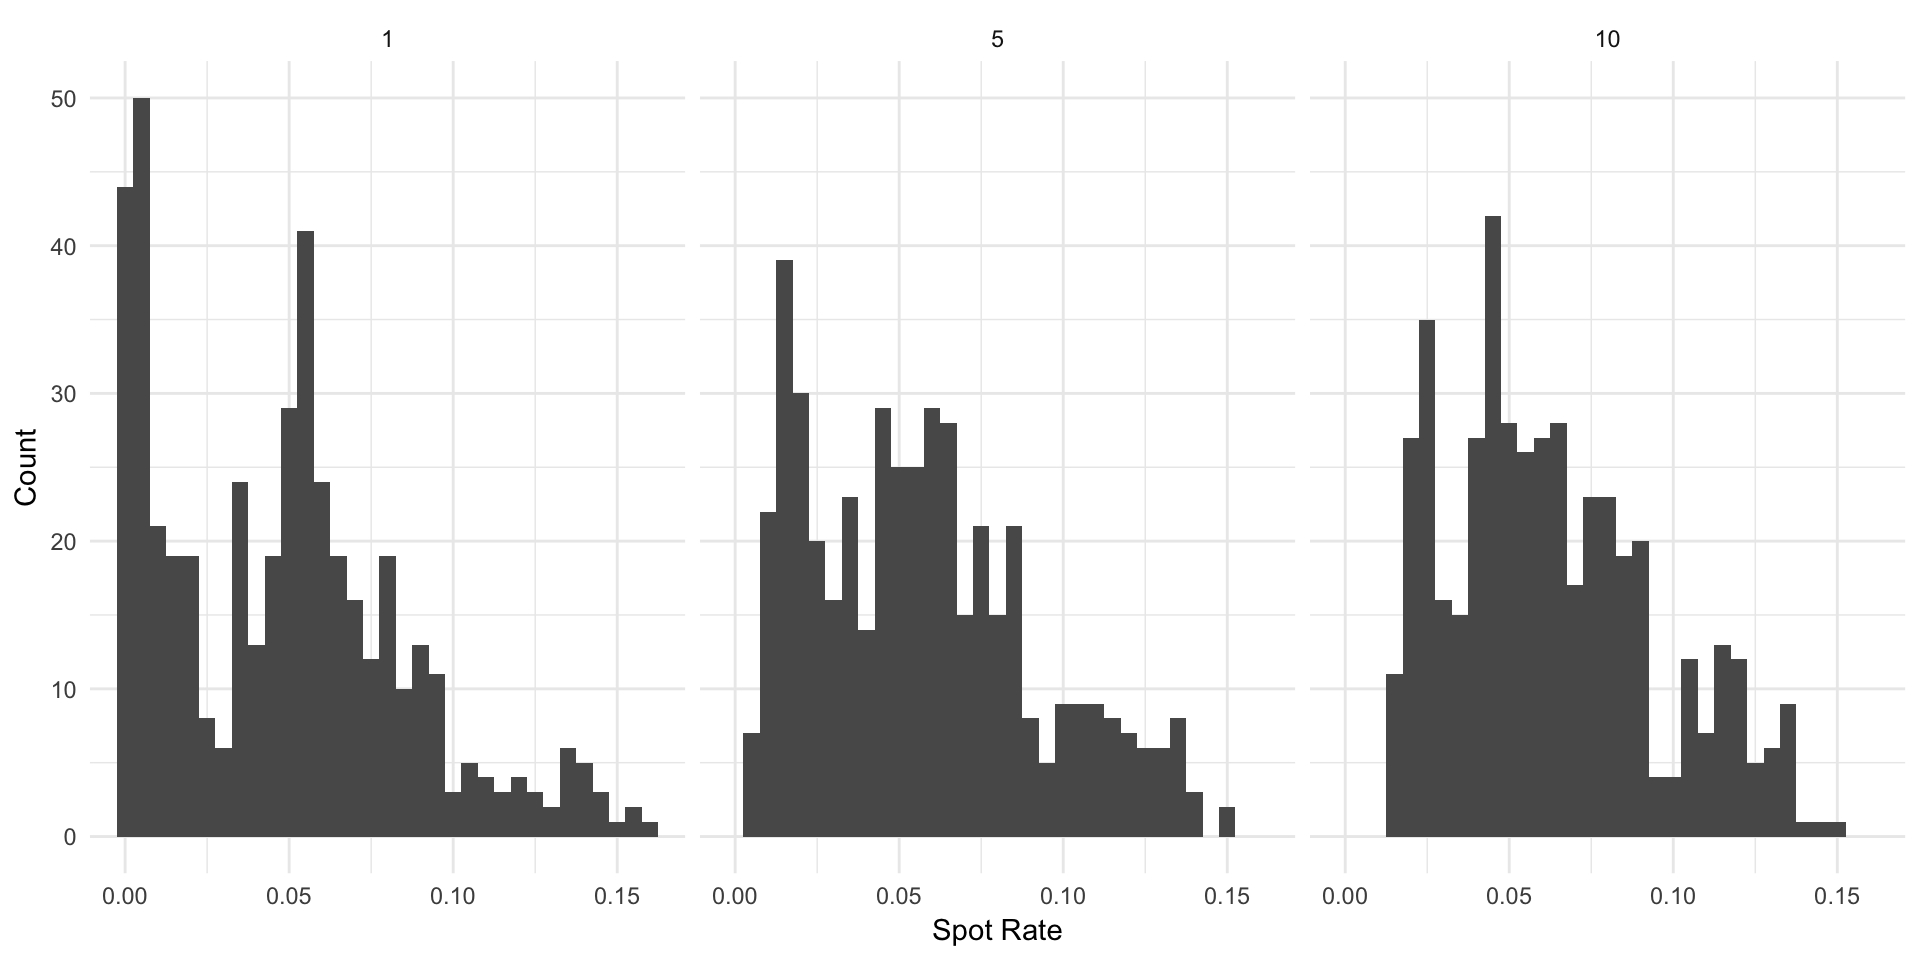
\includegraphics{final-project-book_files/figure-latex/spot-rate-hist-1} 

}

\caption{Spot rate distributions}\label{fig:spot-rate-hist}
\end{figure}

\normalsize

\hypertarget{autocorrelations}{%
\section{Autocorrelations}\label{autocorrelations}}

The first four autocorrelation coefficients of the 3 series are reported
in Table \ref{tab:acf-table}, along with a plot of the ACF for the
entire series in Figure \ref{fig:acf-chart}. Each of the series are
highly autocorrelated, with autocorrelation above 0.6 out past the 25th
lag. By looking at the entire ACF, one can note that the amount of and
persistance of autocorrelation increases in maturity.

\small

\begin{table}[H]

\caption{\label{tab:acf-table}Autocorrelation coefficients for 1, 5, and 10 year spot rates.}
\centering
\begin{tabular}[t]{rrrrr}
\toprule
Maturity & Lag 1 & Lag 2 & Lag 3 & Lag 4\\
\midrule
1 & 0.9878979 & 0.9697433 & 0.9527499 & 0.9411647\\
5 & 0.9911143 & 0.9791933 & 0.9686252 & 0.9599084\\
10 & 0.9906205 & 0.9793246 & 0.9691974 & 0.9606667\\
\bottomrule
\end{tabular}
\end{table}

\normalsize

\small

\begin{figure}[H]

{\centering 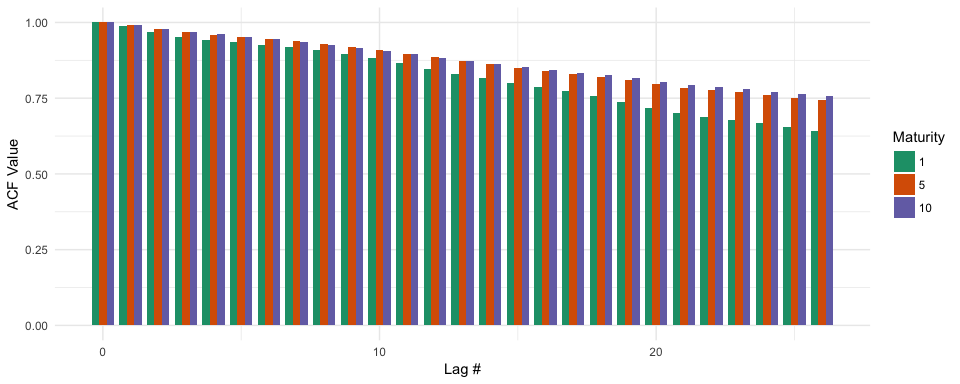
\includegraphics{final-project-book_files/figure-latex/acf-chart-1} 

}

\caption{ACF for the 1, 5, and 10 year spot rates}\label{fig:acf-chart}
\end{figure}

\normalsize

\hypertarget{correlations}{%
\section{Correlations}\label{correlations}}

Correlations between the 1, 5, and 10 year spot rates are reported in
Table \ref{tab:correlations}. It is clear that the the series are
\emph{highly} correlated. This should not be surprising whatsoever.
Intuitively, the 1 year is more correlated with the 5 year than with the
10 year, but the overall correlations are so high that this likely has
no significant meaning.

\small

\begin{table}[H]

\caption{\label{tab:correlations}Correlation coefficients for 1, 5, and 10 year spot rates.}
\centering
\begin{tabular}[t]{rrrr}
\toprule
Maturity & 1 & 5 & 10\\
\midrule
1 & 1.0000000 & 0.9783620 & 0.9539364\\
5 & 0.9783620 & 1.0000000 & 0.9932312\\
10 & 0.9539364 & 0.9932312 & 1.0000000\\
\bottomrule
\end{tabular}
\end{table}

\normalsize

\hypertarget{time-series-visualizations}{%
\section{Time Series Visualizations}\label{time-series-visualizations}}

A look at the time series of the three series confirms the highly
autocorrelated and correlated nature of the three series. 1 year spot
rates are almost always below the longer maturity rates, as one would
expect. Since 2010, 1 year spot rates have been incredibly low, but have
started to pick back up in the last few years.

\small

\begin{figure}[H]

{\centering 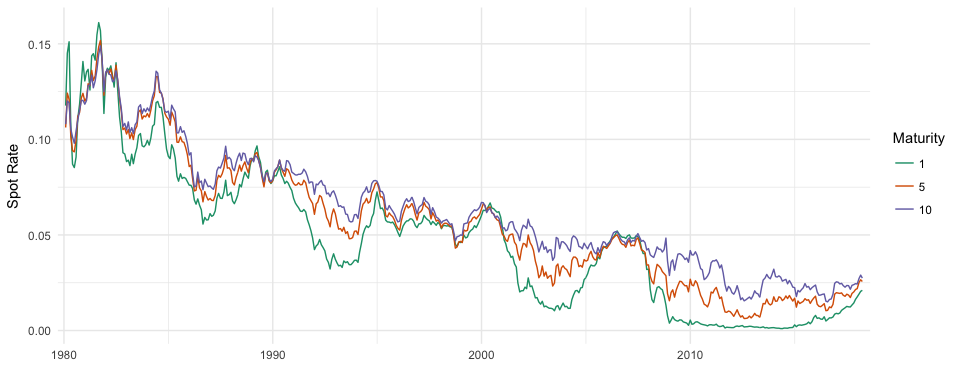
\includegraphics{final-project-book_files/figure-latex/spot-rates-over-time-1} 

}

\caption{A look at the 1, 5, and 10 year spot rates over time}\label{fig:spot-rates-over-time}
\end{figure}

\normalsize

\small

\normalsize

\hypertarget{q2}{%
\chapter{Question 2}\label{q2}}

\textbf{Question:}

\emph{Can the three yield curve factors explain the time-series
variation in spot rates? Regress \(y_t(1)\) on a constant and \(X_t\)
and comment on the regression statistics. Perform the same analysis for
\(y_t(5)\) and \(y_t(10)\).}

\small

\normalsize

In this question, data for the \(y_t(1)\), \(y_t(5)\), and \(y_t(10)\)
spot rates is required along with the yield curve factors, \(X_t\).
These have been calculated in Section \ref{spot-rates} and Section
\ref{yield-curve-factors}, and the results from there are used here.

\small

\normalsize

\hypertarget{regression}{%
\section{Regression}\label{regression}}

The following regression was run on every spot rate series:

\[ y_{t}(n) = \alpha(n) + \beta_1(n) \text{Level}_t + \beta_2(n) \text{Slope}_t + \beta_3(n) \text{Curvature}_t + \epsilon_t(n) \]

Using the concept of multiple models from the book,
\href{http://r4ds.had.co.nz/many-models.html}{\texttt{R\ 4\ Data\ Science}},
implementing these regressions in R is incredibly straightforward. The
general concept involves two steps:

\begin{enumerate}
\def\labelenumi{\arabic{enumi})}
\tightlist
\item
  Split the data set of all 14 maturities into 14 groups, stored in a
  nested data frame.
\item
  For each group, run the linear model above and store the result.
\end{enumerate}

\small

\normalsize

\small

\normalsize

The final result is a compact single data frame that contains the 14
resulting models along with the original data, indexed by the maturity.

\small

\begin{verbatim}
## # A tibble: 14 x 3
##    maturity data               model   
##       <dbl> <list>             <list>  
##  1   0.0833 <tibble [459 x 5]> <S3: lm>
##  2   0.25   <tibble [459 x 5]> <S3: lm>
##  3   0.917  <tibble [459 x 5]> <S3: lm>
##  4   1      <tibble [459 x 5]> <S3: lm>
##  5   2      <tibble [459 x 5]> <S3: lm>
##  6   2.92   <tibble [459 x 5]> <S3: lm>
##  7   3      <tibble [459 x 5]> <S3: lm>
##  8   4.92   <tibble [459 x 5]> <S3: lm>
##  9   5      <tibble [459 x 5]> <S3: lm>
## 10   6.92   <tibble [459 x 5]> <S3: lm>
## 11   7      <tibble [459 x 5]> <S3: lm>
## 12   8      <tibble [459 x 5]> <S3: lm>
## 13   9.92   <tibble [459 x 5]> <S3: lm>
## 14  10      <tibble [459 x 5]> <S3: lm>
\end{verbatim}

\normalsize

\hypertarget{one-year-spot-rate}{%
\section{One Year Spot Rate}\label{one-year-spot-rate}}

As seen in Table \ref{tab:one-year-reg} and Table
\ref{tab:one-year-reg-r2}, all estimates for the 1 year spot rate model
are highly significant, and the Adjusted \(R^2\) is nearing 100\%,
suggesting that the model can explain essentially all of the variation
in the spot rate. Considering that the constructed yield curve factors
include \(y_t(2)\) as the level effect, this should not be surprising as
all of the series are highly correlated. The very high statistic on the
level coefficient supports the claim of its importance.

\small

\begin{table}[H]

\caption{\label{tab:one-year-reg}Regression results: One year spot}
\centering
\begin{tabular}[t]{lrrrr}
\toprule
Term & Estimate & Standard Error & Statistic & P-Value\\
\midrule
Intercept & 0.001014021 & 0.0001280165 & 7.921022 & 1.8e-14\\
Level & 0.989941953 & 0.0015226534 & 650.142657 & 0.0e+00\\
Slope & 0.264774017 & 0.0034323179 & 77.141460 & 0.0e+00\\
Curvature & -0.428350107 & 0.0057618892 & -74.341954 & 0.0e+00\\
\bottomrule
\end{tabular}
\end{table}

\normalsize

\small

\begin{table}[H]

\caption{\label{tab:one-year-reg-r2}Regression $R^2$: One year spot}
\centering
\begin{tabular}[t]{rrr}
\toprule
R Squared & R Squared Adj & Residual Std Error\\
\midrule
0.9995224 & 0.9995193 & 0.0008223\\
\bottomrule
\end{tabular}
\end{table}

\normalsize

A chart of the realized VS predicted time series for each model confirms
how well the variation is explained, with essentailly perfect matching
of the realized series. It is important to remember that this model is
not predicting out-of-sample future rates, and is simply used to gather
intuition about past rates. Nevertheless, it is interesting to see how
well the yield curve factors explain the variation.

\small

\begin{figure}[H]

{\centering 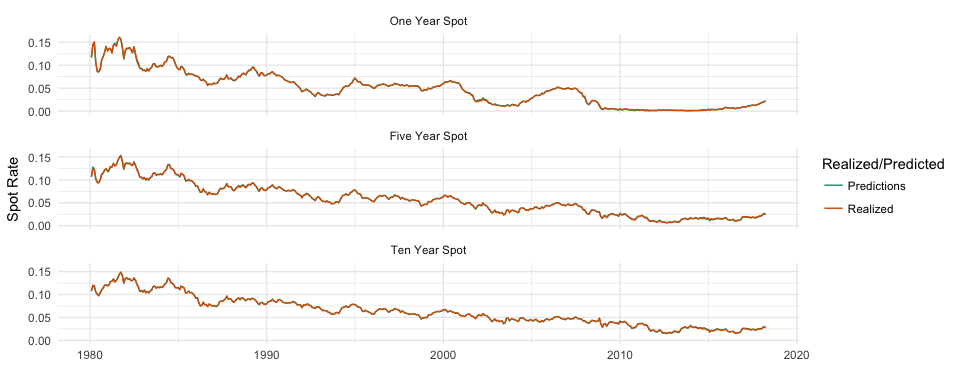
\includegraphics{final-project-book_files/figure-latex/spot-rate-reg-chart-1} 

}

\caption{In-sample realized VS predicted spot rate series}\label{fig:spot-rate-reg-chart}
\end{figure}

\normalsize

\hypertarget{five-year-spot-rate}{%
\section{Five Year Spot Rate}\label{five-year-spot-rate}}

The model for the 5-year rate is similar to the 1-year rate in terms of
explanatory power. The level coefficient is slightly higher than for the
1-year, and is \textgreater{}1, which makes sense considering that the
5-year is generally higher than the 2-year spot rate used to represent
the level effect. The slope is more than triple that of the 1-year,
suggesting that an increase in the slope has a larger impact on the
value of the 5-year curve than it does on the 1-year.

\small

\begin{table}[H]

\caption{\label{tab:five-year-reg}Regression results: Five year spot}
\centering
\begin{tabular}[t]{lrrrr}
\toprule
Term & Estimate & Standard Error & Statistic & P-Value\\
\midrule
Intercept & -0.001326488 & 0.0001178948 & -11.25146 & 0\\
Level & 1.010756975 & 0.0014022642 & 720.80351 & 0\\
Slope & 0.862622600 & 0.0031609403 & 272.90063 & 0\\
Curvature & -0.237885069 & 0.0053063231 & -44.83049 & 0\\
\bottomrule
\end{tabular}
\end{table}

\normalsize

\small

\begin{table}[H]

\caption{\label{tab:five-year-reg-r2}Regression $R^2$: Five year spot}
\centering
\begin{tabular}[t]{rrr}
\toprule
R Squared & R Squared Adj & Residual Std Error\\
\midrule
0.9995226 & 0.9995194 & 0.0007572\\
\bottomrule
\end{tabular}
\end{table}

\normalsize

\hypertarget{ten-year-spot-rate}{%
\section{Ten Year Spot Rate}\label{ten-year-spot-rate}}

Finally, the 10-year model performs similarly to the 1 and 5-year
models. One interesting thing to note about the 10-year model is that
the sign on the curvature coefficient is opposite that of the 1 and
5-year models.

\small

\begin{table}[H]

\caption{\label{tab:ten-year-reg}Regression results: Ten year spot}
\centering
\begin{tabular}[t]{lrrrr}
\toprule
Term & Estimate & Standard Error & Statistic & P-Value\\
\midrule
Intercept & 0.001285415 & 9.632731e-05 & 13.34424 & 0\\
Level & 0.990119282 & 1.145736e-03 & 864.17722 & 0\\
Slope & 1.041806029 & 2.582683e-03 & 403.38126 & 0\\
Curvature & 0.101703126 & 4.335593e-03 & 23.45772 & 0\\
\bottomrule
\end{tabular}
\end{table}

\normalsize

\small

\begin{table}[H]

\caption{\label{tab:ten-year-reg-r2}Regression $R^2$: Ten year spot}
\centering
\begin{tabular}[t]{rrr}
\toprule
R Squared & R Squared Adj & Residual Std Error\\
\midrule
0.9996166 & 0.9996141 & 0.0006187\\
\bottomrule
\end{tabular}
\end{table}

\normalsize

\hypertarget{decomposing-the-spot-curve}{%
\section{Decomposing the Spot Curve}\label{decomposing-the-spot-curve}}

Although not specifically asked for, it might be interesting to
decompose and plot the spot curve at a few particular points in time.
The procedure for this involves the following manipulations:

\begin{enumerate}
\def\labelenumi{\arabic{enumi})}
\tightlist
\item
  For month \texttt{m}, extract the spot rate at every available
  maturity for that month.
\item
  For month \texttt{m}, filter the yield curve factors down to that
  month, and multiply each maturity's regression coefficients by the
  corresponding yield curve factor. This gives the contribution of each
  factor for that month and each maturity.
\item
  Join the two data sets and chart them to view the decomposed spot rate
  for any month.
\end{enumerate}

\small

\normalsize

\small

\normalsize

\small

\normalsize

\small

\normalsize

This procedure was streamlined into a single function, parameterized by
the month to allow for easy plotting and comparison of multiple months.
For example, the decomposed spot curve for January 2012 and January 1981
are shown side-by-side in Figure \ref{fig:decomposed-spot}. January of
1981 was definitely an interesting time period! The spot rate is
essentially inverted, with lower maturity bonds having higher spot rates
than longer maturity bonds.

\small

\begin{figure}[H]

{\centering 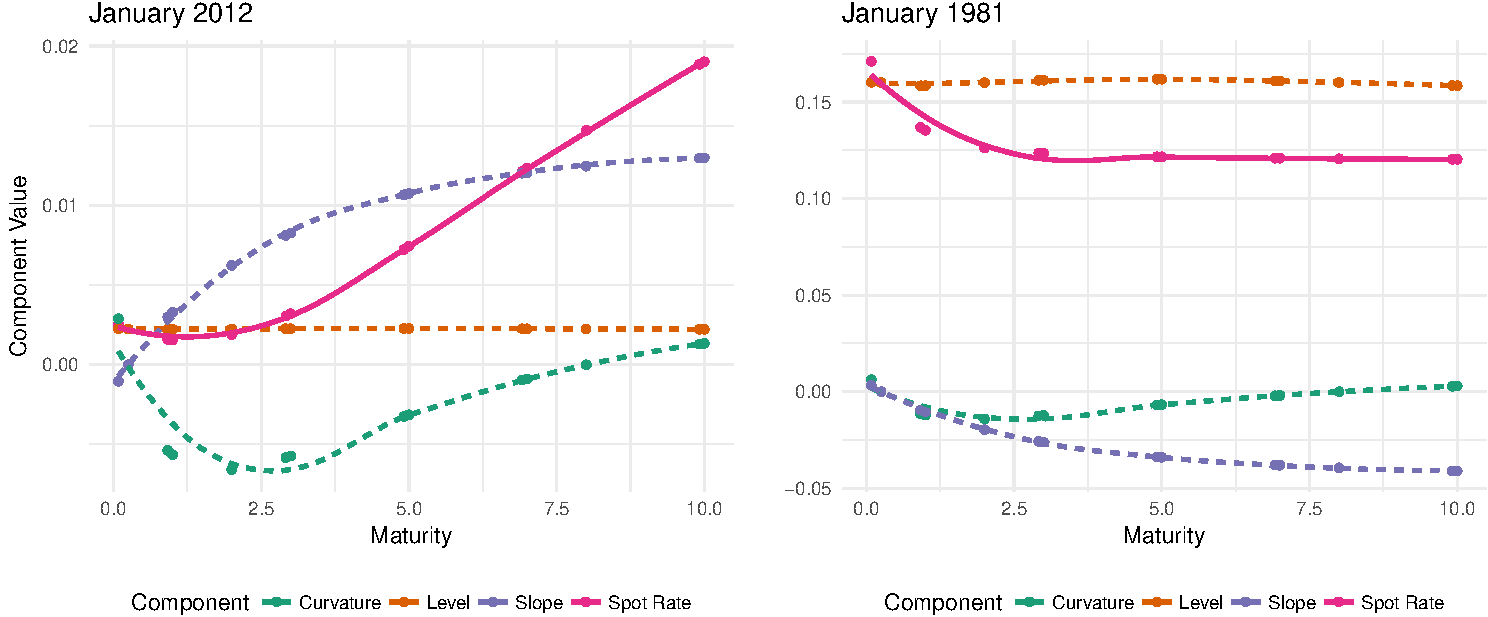
\includegraphics{final-project-book_files/figure-latex/decomposed-spot-1} 

}

\caption{Decomposed spot rate for January of 2012 and 1981}\label{fig:decomposed-spot}
\end{figure}

\normalsize

\hypertarget{coef-stability}{%
\section{Coefficient Stability}\label{coef-stability}}

Another question worth asking is how stable the coefficients are
throughout time. We can test this by running the same regression as
before, but with a \emph{rolling window}. This works by calculating the
regression
\texttt{spot\_rate\ \textasciitilde{}\ level\ +\ slope\ +\ curvature}
for the first 100 months, then shifting forward 1 month and dropping the
last day, calculating the regression again, and repeating this for the
length of the series. The \texttt{rsample} package provides a number of
helpers for doing analysis exactly like this. The procedure for this is:

\begin{enumerate}
\def\labelenumi{\arabic{enumi})}
\tightlist
\item
  Split the data into 14 nested groups by maturity, as done in Section
  \ref{regression}.
\item
  Further split each of the 14 groups into 359 rolling subsets of 100
  days each using \texttt{rolling\_origin()} from \texttt{rsample}.
\item
  For each maturity, and for each rolling split, run the regression from
  \ref{regression}. This results in 5026 regressions, which, on this
  4-core computer, can be run in parallel in \textasciitilde{}8 seconds.
\end{enumerate}

\small

\normalsize

\small

\normalsize

\small

\normalsize

When the procedure has been run, a natural next step is to pick some of
the 14 maturities and look at the stability of each coefficient over
time. For example, the 1, 5, and 10 year coefficients over time are
shown side-by-side in Figure \ref{fig:coef-stability}. Most of the
coefficients are fairly stable over time, with the exception of
curvature. The curvature of the 1 year has begun to rise up from -0.5 to
around -0.25 in recent years. This change over time is not refected in
the static -0.428 curvature estimate we get from running the model over
the full time period, and might offer other interesting insights or
opportunities for trading strategies. The 10 year curvature coefficient
follows a similar pattern, but the 5 year curvature follows the opposite
trend, decreasing in recent years.

\small

\normalsize

\small

\begin{figure}[H]

{\centering 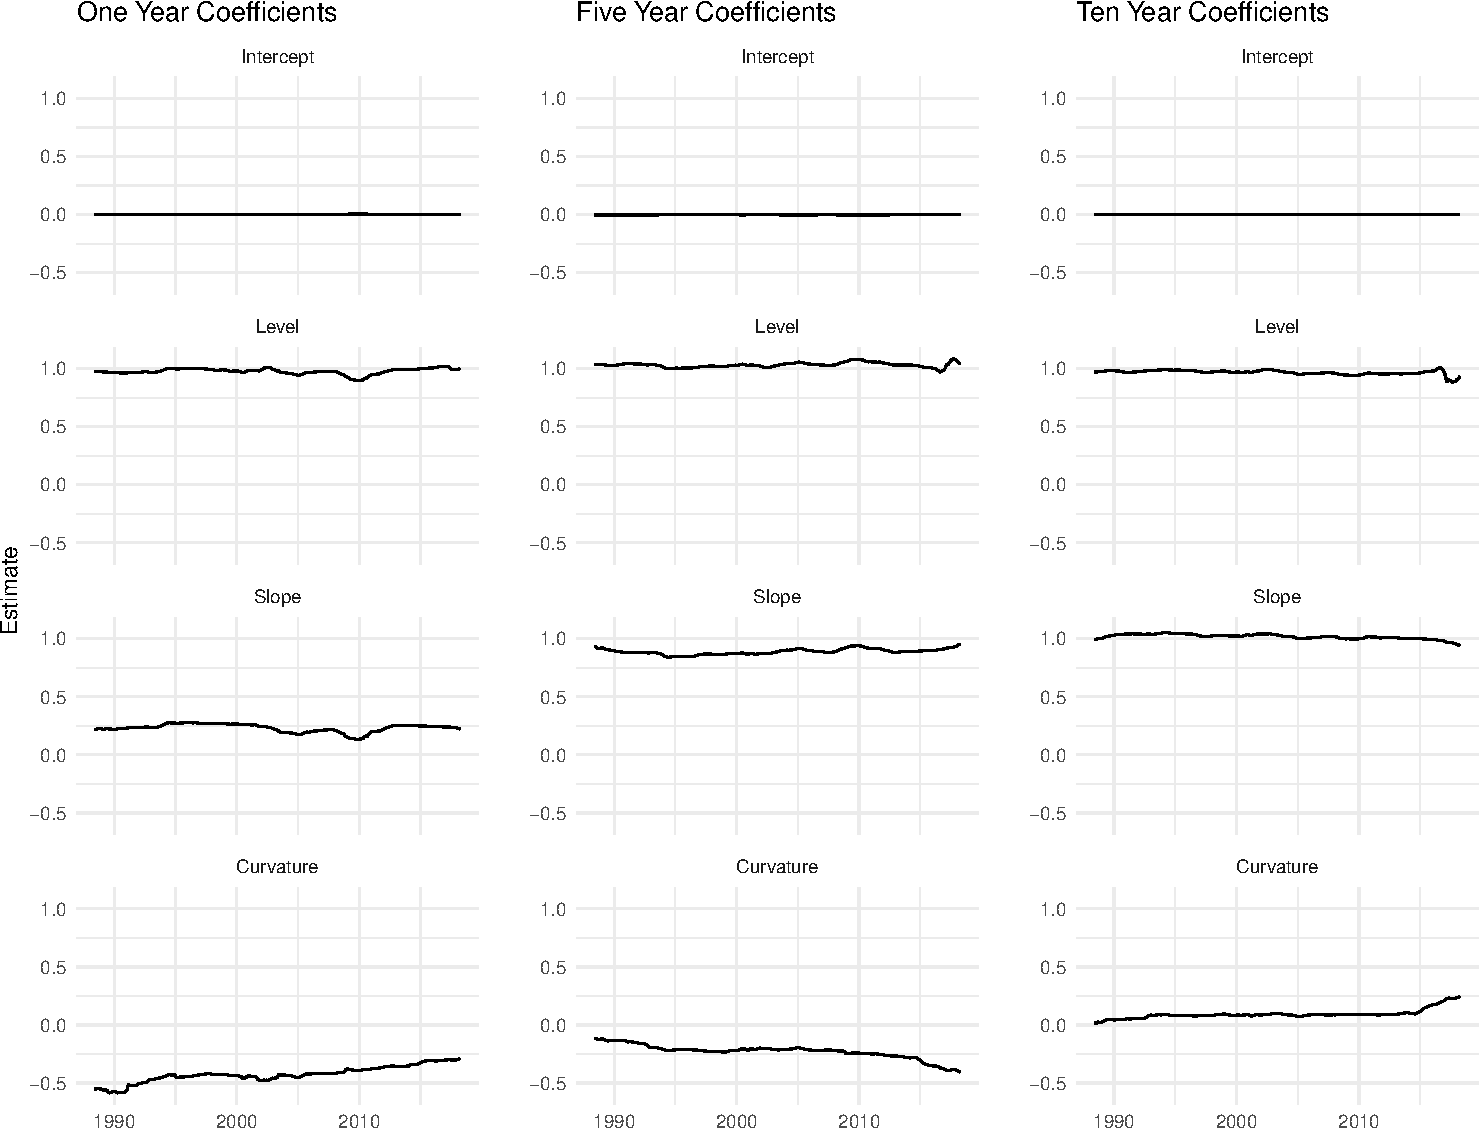
\includegraphics{final-project-book_files/figure-latex/coef-stability-1} 

}

\caption{Coefficient stability for 1, 5, and 10 year spot rates. 100 month rolling window.}\label{fig:coef-stability}
\end{figure}

\normalsize

\small

\normalsize

\hypertarget{q3}{%
\chapter{Question 3}\label{q3}}

\textbf{Question:}

\emph{Perform the ``out-of-sample'' hedging exercises where \(n_h = 3\).
Split the sample into two halves, such that \(T_0 = 2T\). Begin with the
\(T\)-th month, calculate \(w_T(1)\), \(w_T(5)\), and \(w_T(10)\) for
each hedging strategy, and save \(\epsilon_{T+\Delta}(n_h)\). Move
forward and repeat the process each month, and calculate the root mean
squared hedging error (RMSHE) for each strategy:}

\[ RMSHE = [\frac{1}{T} \sum{\epsilon_{t+\Delta}(n_h)}]^{0.5} \]

\emph{Report your results and evaluate the performance of the hedging
strategies.}

\textbf{Implementation details:}

This chapter is broken into:

\begin{itemize}
\tightlist
\item
  3 sections devoted to creating the modeling functions
\item
  1 section for creating a hedging error calculation function
\item
  1 section for creating an ``interface'' to the models and error
  calculations
\item
  1 section for running the models through the interface
\item
  1 section for reviewing model performance
\end{itemize}

\small

\normalsize

The data for the \(y_t(1)\), \(y_t(3)\), \(y_t(5)\), \(y_t(7)\), and
\(y_t(10)\) spot rates is required to calculate the durations for the
zero coupon bonds used in the hedging exercises. Also required are the
yield curve factors and excess returns. These have all been calculated
in Section \ref{rates}, and the results from there are used.

\small

\normalsize

The models developed below will be structured in a way so that they can
all be fed with data from the same data set. To accomplish the rolling
out-of-sample technique, the \texttt{rsample} package was used.
Specifically, the \texttt{rolling\_origin()} function was utilized which
allows easy splitting of data into rolling sets of 230 months, which is
the \texttt{T} value corresponding to half of the data.

\small

\normalsize

\small

\normalsize

\small

\normalsize

\small

\normalsize

\hypertarget{modified-macaulay-duration}{%
\section{Modified / Macaulay
Duration}\label{modified-macaulay-duration}}

The first two strategies involve creating duration matched barbells
using 1-year and 10-year zero coupon bonds to match the duration of a
3-year or 7-year bullet. Since the strategies are essentially the same,
one modeling function is used for both, \texttt{model\_duration()}, with
an argument to select whether to use modified or macaulay duration. The
duration is calculated using the \texttt{duration()} function in the
\texttt{ratekit} package and the barbell weights are calculated with the
\texttt{barbell\_weights()} function.

The function is created in such a way that it accepts a single split
from the total data frame, and calculates the weights for just that one
split. The weight for a 5-year zero is included to be consistent with
the other models, but is set to \texttt{0}.

\small

\normalsize

\hypertarget{simple-regression-based-hedging}{%
\section{Simple Regression Based
Hedging}\label{simple-regression-based-hedging}}

The regression based hedging method involves the regression:

\[ ER_t(n_h) = w_t(1) ER_t(1) + w_t(5) ER_t(5) + w_t(10) ER_t(10) + u_t(n_h) \]

The R function \texttt{lm()} is used to run the regression, and the
weights are extracted and returned in the same format as the duration
models. This is all wrapped into a modeling function,
\texttt{model\_regression()}.

\small

\normalsize

\hypertarget{multiplicative-regression-hedging}{%
\section{Multiplicative Regression
Hedging}\label{multiplicative-regression-hedging}}

The multiplicative regression follows the model:

\[ ER_t(n_h) = \theta_t(1; X_{t-\Delta}) ER_t(1) + \theta_t(5; X_{t-\Delta}) ER_t(5) + \theta_t(10; X_{t-\Delta}) ER_t(10) + u_t(n_h) \]
where \(\theta_t(n; X_{t-\Delta})\) depends on the yield curve factors
as:

\[ \theta_t(n; X_{t-\Delta}) = a_t(n) + b_t(n) \text{Level}_{t-\Delta} + c_t(n) \text{Slope}_{t-\Delta} + d_t(n) \text{Curvature}_{t-\Delta} \]

Once the models are fit, the weights at time \(t\) can be calculated as
\(\theta_t\) values using the yield curve factors at \(t\):

\[ 
w_t(1) = \theta_t(1; X_t) \\ 
w_t(5) = \theta_t(5; X_t) \\ 
w_t(10) = \theta_t(10; X_t)
\]

The entire procedure is wrapped into
\texttt{model\_multiplicative\_regression()}, which, consistent with the
other \texttt{model\_*()} functions developed so far, accepts a single
rolling split, along with the type of bullet (3 or 7-year), and returns
the weights.

\small

\normalsize

\hypertarget{error-calculation}{%
\section{Error Calculation}\label{error-calculation}}

Hedging error for the weights set at time \(t\) are calculated at time
\(t+\Delta\) as:

\[ \epsilon_{t+\Delta} = w_t(1) ER_{t+\Delta}(1) + w_t(5) ER_{t+\Delta}(5) + w_t(10) ER_{t+\Delta}(10) \]
These weights are then aggregated using RMSHE to determine overall model
performance.

\small

\normalsize

\hypertarget{model-selection-interface}{%
\section{Model Selection Interface}\label{model-selection-interface}}

A practical way to call all of the above models would be through an
interface function that take as parameters: the data, the model to run,
and the bullet to hedge against. Such a function was developed, and
returns a data frame of the model type, the bullet used, the date of the
error calculation, the weights, and the hedging errors.

\small

\normalsize

\small

\normalsize

\small

\normalsize

\small

\normalsize

\hypertarget{model-application}{%
\section{Model Application}\label{model-application}}

\small

\normalsize

Finally, a data frame of function calls and parameter sets is created to
easily iterate over all of the models. This data frame has a very
compact form:

\small

\begin{Shaded}
\begin{Highlighting}[]
\NormalTok{invokable}
\end{Highlighting}
\end{Shaded}

\begin{verbatim}
## # A tibble: 8 x 2
##   f           params    
##   <chr>       <list>    
## 1 apply_model <list [3]>
## 2 apply_model <list [3]>
## 3 apply_model <list [3]>
## 4 apply_model <list [3]>
## 5 apply_model <list [3]>
## 6 apply_model <list [3]>
## 7 apply_model <list [3]>
## 8 apply_model <list [3]>
\end{verbatim}

\normalsize

The first column contains the function interface,
\texttt{apply\_model()}. Each element of the \texttt{params} column
contains the data to be used in the model, the model type, and the
bullet to hedge against.

\small

\begin{Shaded}
\begin{Highlighting}[]
\NormalTok{invokable}\OperatorTok{$}\NormalTok{params[[}\DecValTok{1}\NormalTok{]]}
\end{Highlighting}
\end{Shaded}

\begin{verbatim}
## $.data
## # Rolling origin forecast resampling 
## # A tibble: 229 x 2
##   splits       id      
##   <list>       <chr>   
## 1 <S3: rsplit> Slice001
## 2 <S3: rsplit> Slice002
## 3 <S3: rsplit> Slice003
## 4 <S3: rsplit> Slice004
## 5 <S3: rsplit> Slice005
## # ... with 224 more rows
## 
## $model
## [1] "modified_duration"
## 
## $bullet
## [1] "3"
\end{verbatim}

\normalsize

\hypertarget{model-results}{%
\section{Model Results}\label{model-results}}

Table \ref{tab:hedging-results} displays the RMSHE results from each
model. The regression methods significantly outperformed the duration
based models, with much lower RMSHE. Among the duration models, Macaulay
duration did marginally better, but the statistical significance is
likely negligible. Among the regression models, the multiplicative
regression did slightly better than the simple regression with the
3-year bullet and slightly worse with the 7-year bullet. The results are
so close, however, that I am inclined to conclude that the simpler
regression model is the best and most parsimonious model of the four.
There is little to indicate that longer maturity bullets are harder to
hedge than shorter maturity bullets. In fact, with the regression
models, the opposite seems to be true.

\small

\begin{table}[H]

\caption{\label{tab:hedging-results}Hedging Model Results}
\centering
\begin{tabular}[t]{llr}
\toprule
Model & Bullet & RMSHE\\
\midrule
Macaulay & 3 & 0.0038994\\
Macaulay & 7 & 0.0039961\\
Modified & 3 & 0.0039390\\
Modified & 7 & 0.0040058\\
Multipl. Regression & 3 & 0.0008060\\
\addlinespace
Multipl. Regression & 7 & 0.0007763\\
Regression & 3 & 0.0008178\\
Regression & 7 & 0.0007663\\
\bottomrule
\end{tabular}
\end{table}

\normalsize

\small

\normalsize

Because a rolling model was fit, a similar analysis can be performed as
Section \ref{coef-stability} where the stability of the coefficients
over time was analyzed. In this case, the assignment of hedging weights
by the models over time can be analyzed rather than just the
coefficients. Some interesting insights can be gathered from Figure
\ref{fig:weight-stability}. Keeping in mind that duration models are
\emph{only} allowed to assign weight to a 1 year and 10 year zero, it is
interesting to see how stagnant the weighting is between the 1 year and
10 year. The fact that the model essentially does not have the
flexibility to vary the weights much over time likely contributes to its
poor performance. The duration model also never shorts, which likely
helps the regression models. The weightings in the duration models do
make sense, with more than 50\% being assigned to the 1-year bond to
hedge the 3-year bullet, and more than 50\% being assigned to the
10-year the hedge the 7-year bullet. In the regression models, there is
an implicit risk free instrument that weight can be assigned to, so a
4th row in the figure is included to incorporate that. The simple
regression model only shifts weights around in periods of high stress,
2001 and the jump around 2008 being two examples, but even so, the
weightings are surprisingly stable over time. This is especially
apparent when contrasted with the multiplicative regression. Weights are
highly varied over time, but the performance gain for this is limited as
seen in the RMSHE results, questioning the need for the complex model.

\small

\begin{figure}[H]

{\centering 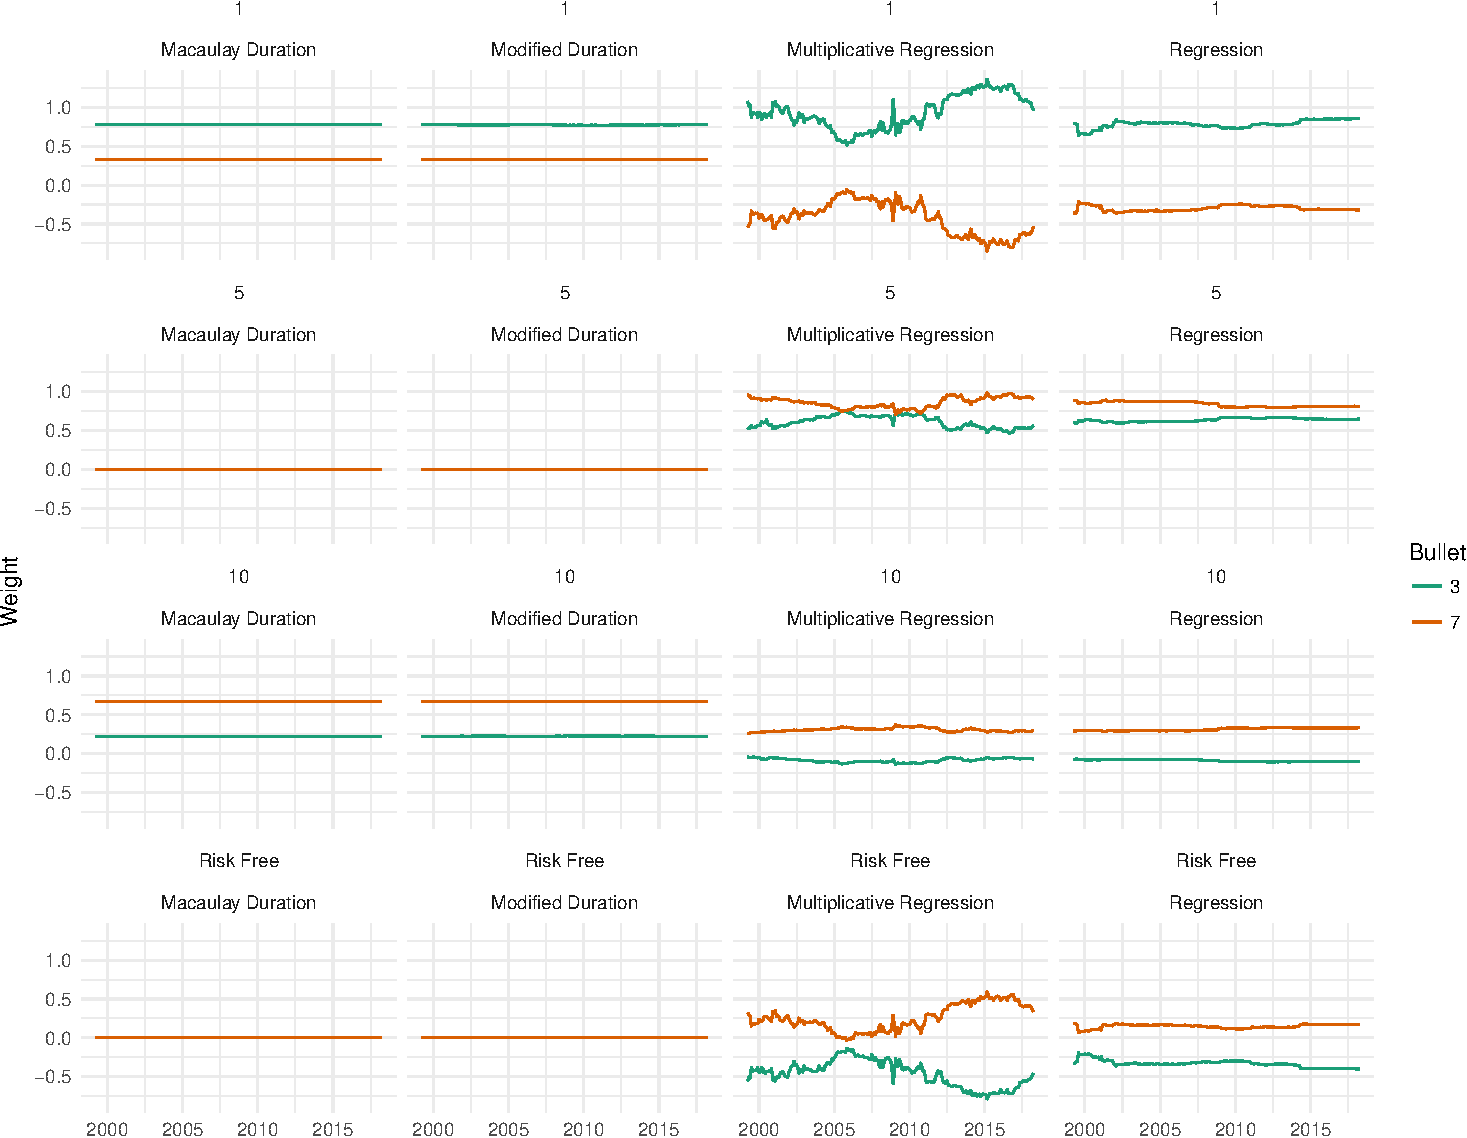
\includegraphics{final-project-book_files/figure-latex/weight-stability-1} 

}

\caption{Hedging weight assignment over time}\label{fig:weight-stability}
\end{figure}

\normalsize

Another way to view the weights over time is by stacking them. This is
done in Figure \ref{fig:stacked-weight-stability} and provides another
unique view into the change in the total weight distribution over time.
This view confirms the stagnant weights in the duration models, but also
offers some other new insights. In the regression models, hedging the
3-year bullet requires shorting the 10-year and the risk free, while
hedging the 7-year bullet only required hedging the 1-year bond. This
view also further demonstrates the wild swings in the multiplicative
regression, for questionable performance gains.

\small

\begin{figure}[H]

{\centering 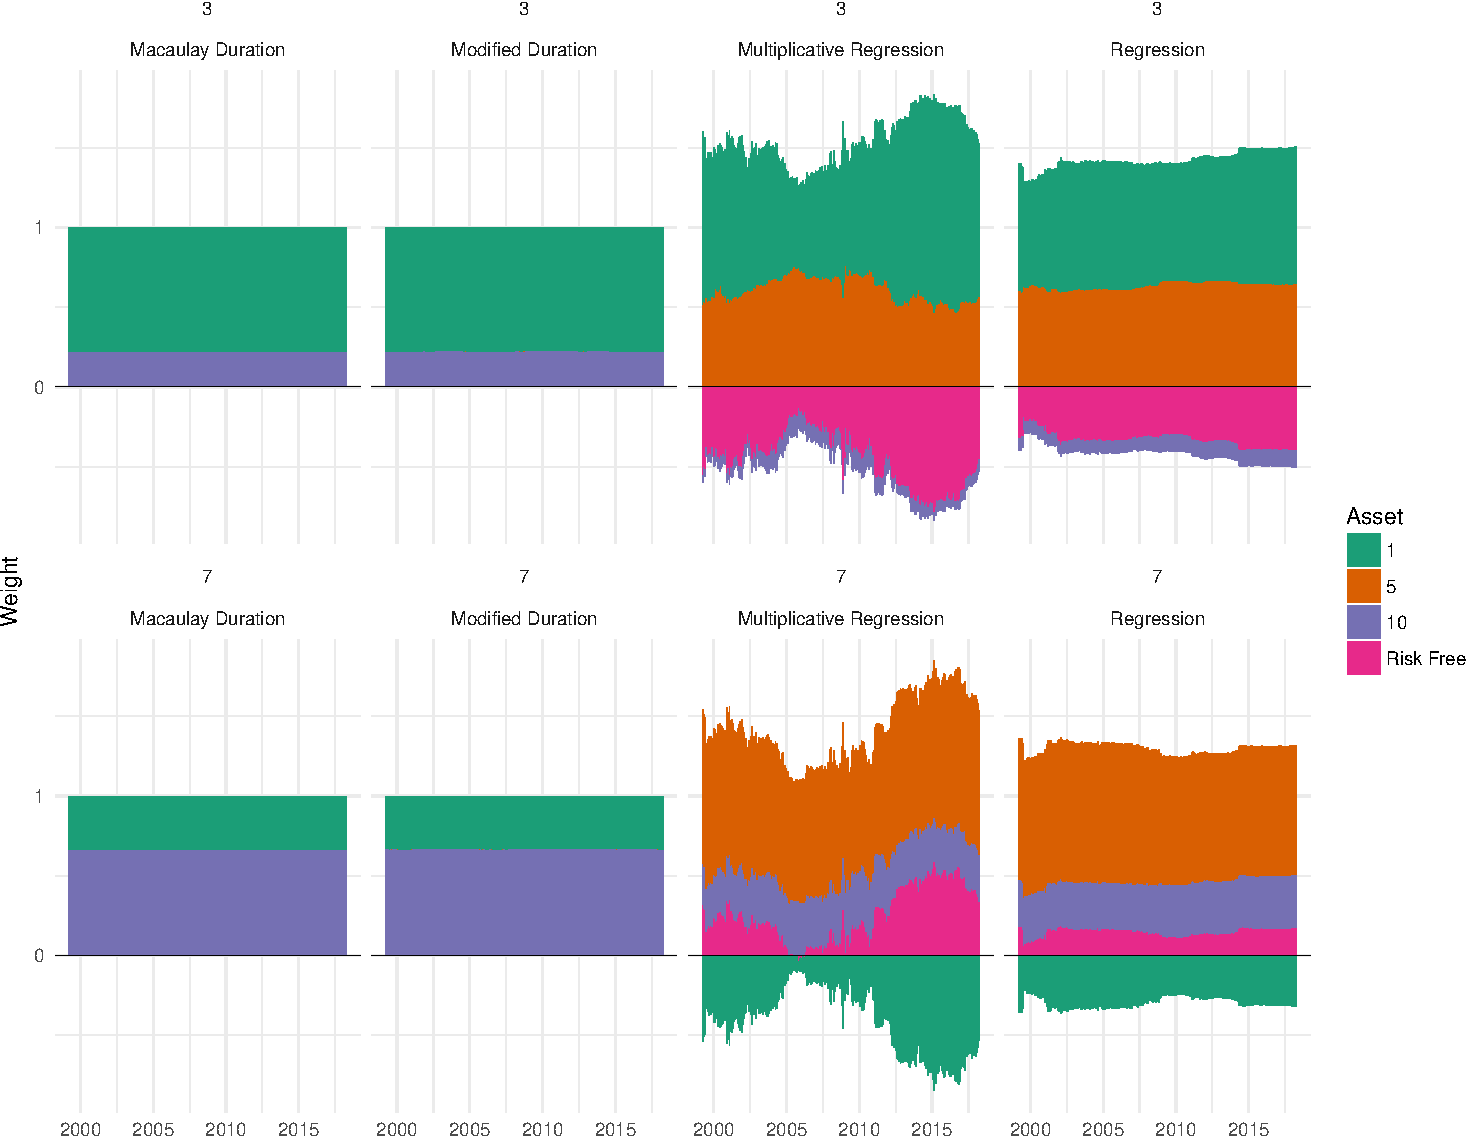
\includegraphics{final-project-book_files/figure-latex/stacked-weight-stability-1} 

}

\caption{Stacked weight assignment over time}\label{fig:stacked-weight-stability}
\end{figure}

\normalsize

\small

\normalsize

\hypertarget{conclusion}{%
\chapter{Conclusion}\label{conclusion}}

In this project, spot rates from the Federal Reserve were analyzed along
with their corresponding zero prices and returns over time. In addition,
multiple hedging models were implemented and analyzed. The simple
regression hedging model outperformed the two duration models, and was
on par with the much more complicated multiplicative regression model.
This leads me to conclude that the simple regression model is the most
useful out of the four.

I was particularly impressed with how well the yield curve factors
explained the variation in the rates for other maturities. Using linear
combinations of certain maturity spot rates seems to create powerful
explanatory variables for other maturities.

Further research could be done by including transactions costs in
hedging performance calculations. This would likely penalize the
multiplicative regression even further. Additionally, one could include
thresholds that had to be hit before a certain recommended change in the
weights was actually made. This could combat the transaction costs and
would benefit the simple regression method along with the duration
methods.

\bibliography{book.bib,packages.bib}


\end{document}
